\documentclass{article}
\usepackage{tikz}
\usetikzlibrary{positioning,shapes,arrows,fit}

\begin{document}

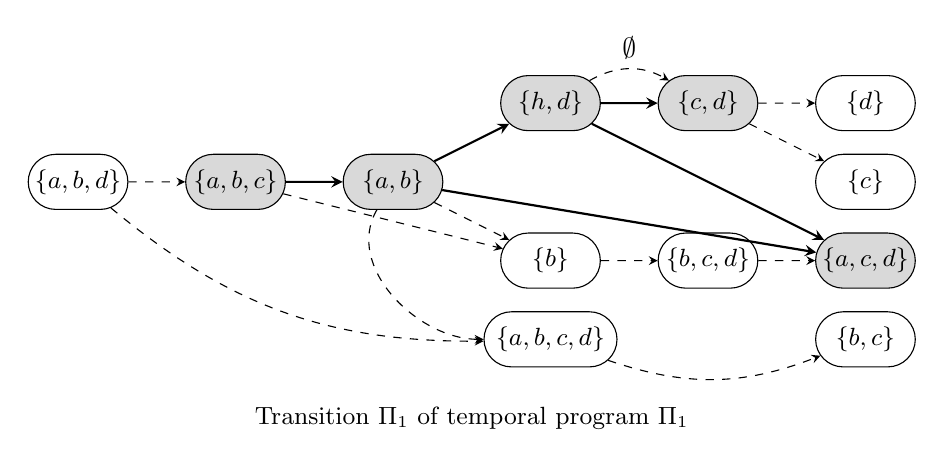
\begin{tikzpicture}[
    node distance=1.5cm,
    state/.style={
        rounded rectangle,
        draw=black,
        minimum height=0.7cm,
        minimum width=1.5cm,
        font=\small
    },
    gray state/.style={
        state,
        fill=gray!30
    },
    solid arrow/.style={
        ->,
        >=stealth,
        thick
    },
    dashed arrow/.style={
        ->,
        >=stealth,
        dashed
    }
]

% Nodes
\node[state] (abd) at (0,0) {$\{a,b,d\}$};
\node[gray state] (abc) at (2,0) {$\{a,b,c\}$};
\node[gray state] (ab) at (4,0) {$\{a,b\}$};
\node[gray state] (hd) at (6,1) {$\{h,d\}$};
\node[gray state] (cd) at (8,1) {$\{c,d\}$};
\node[state] (d) at (10,1) {$\{d\}$};
\node[state] (c) at (10,0) {$\{c\}$};
\node[state] (b) at (6,-1) {$\{b\}$};
\node[state] (bcd) at (8,-1) {$\{b,c,d\}$};
\node[gray state] (acd) at (10,-1) {$\{a,c,d\}$};
\node[state] (abcd) at (6,-2) {$\{a,b,c,d\}$};
\node[state] (bc) at (10,-2) {$\{b,c\}$};

% Solid arrows (representing transitions in solutions of length 4)
\draw[solid arrow] (abc) -- (ab);
\draw[solid arrow] (ab) -- (hd);
\draw[solid arrow] (hd) -- (cd);
\draw[solid arrow] (hd) -- (acd);
\draw[solid arrow] (ab) -- (acd);

% Dashed arrows (other transitions)
\draw[dashed arrow] (abd) -- (abc);
\draw[dashed arrow] (abc) -- (b);
\draw[dashed arrow] (ab) -- (b);
\draw[dashed arrow] (cd) -- (d);
\draw[dashed arrow] (cd) -- (c);
\draw[dashed arrow] (b) -- (bcd);
\draw[dashed arrow] (bcd) -- (acd);
\draw[dashed arrow] (abd) to[bend right=20] (abcd);
\draw[dashed arrow] (abcd) to[bend right=20] (bc);
\draw[dashed arrow] (ab) to[out=240,in=180] (abcd);
\draw[dashed arrow] (hd) to[out=30,in=150] node[above] {$\emptyset$} (cd);

% Add label for the transition graph
\node[font=\small] at (5,-3) {Transition $\graph{\Pi_1}$ of temporal program $\Pi_1$};

\end{tikzpicture}

\end{document}